%%%%%%%%%%%%%%%%%%%%%%%%%%%%%%%%%%%%%%%%
%%%%%%%%%%%%%%%%%%%%%%%%%%%%%%%%%%%%%%%%

% This is a template for usage prior to journal submission.
% Author: Maximilian Linde
% E-mail: m.linde@rug.nl

%%%%%%%%%%%%%%%%%%%%%%%%%%%%%%%%%%%%%%%%
%%%%%%%%%%%%%%%%%%%%%%%%%%%%%%%%%%%%%%%%

\documentclass[meta, authordate]{jote-new-article}

% \usepackage[english]{babel}
% \usepackage[utf8]{inputenc}
% \usepackage[T1]{fontenc}
\usepackage{amsmath}
% \usepackage{amsfonts}
% \usepackage{mathtools}
% \usepackage{amssymb}
% \usepackage{graphicx}
\usepackage{multirow}
% \usepackage[style=apa,sortcites=true,sorting=nyt,backend=biber]{biblatex}
% \usepackage{csquotes}
% \usepackage{hyperref}
\usepackage[most]{tcolorbox}

\DeclareLanguageMapping{american}{american-apa}

\addbibresource{references.bib}
\addbibresource{references_mmp.bib}

% Revisions in pdf
\definecolor{forestgreen}{rgb}{0.13, 0.55, 0.13}
\newcommand{\revise}[1]{\textcolor{forestgreen}{\ifhmode\hskip0pt\relax\fi#1}}
\newcommand{\remove}[1]{\textcolor{red}{\ifhmode\hskip0pt\relax\fi#1}}
% \renewcommand{\revise}[1]{\textcolor{black}{\ifhmode\hskip0pt\relax\fi#1}} % Uncomment to show revisions in normal font.
% \renewcommand{\remove}[1]{} % Uncomment to remove removals.

%%%%%%%%%%%%%%%%%%%%%%%%%%%%%%%%%%%%%%%%
%%%%%%%%%%%%%%%%%%%%%%%%%%%%%%%%%%%%%%%%
\paperdoi{10.36850/mr10}
\paperreceived{December 20, 2022}
\paperaccepted{October 27, 2023}
\paperpublished{March 1, 2024}
\paperpublisheddate{2024-03-01}

   \jname{Journal of Trial \& Error}
   \jyear{2024}
   \jwebsite{https://journal.trialanderror.org}
\jotetitle{Reputation Without Practice? A Dynamic Computational Model of the Unintended Consequences of Open Scientist Reputations}

% \shorttitle{}

\runningauthor{Linde et al.}

\author[1]{Maximilian~Linde\orcid{0000-0001-8421-090X}}
\author[1,2]{Merle-Marie~Pittelkow\orcid{0000-0002-7487-7898}}
\author[3]{\mbox{Nina~R.~Schwarzbach\orcid{0000-0002-0129-0340}}}
\author[1]{Don~van~Ravenzwaaij\orcid{0000-0002-5030-4091}}

\affil[1]{Unit of Psychometrics and Statistics, Department of Psychology, Faculty of Behavioural and Social Sciences, University of Groningen, Groningen, The Netherlands}
\affil[2]{QUEST Center for Responsible Research, Berlin Institute of Health at Charit{\'{e}}, Berlin, Germany}
\affil[3]{Unit of Clinical and Developmental Neuropsychology, Department of Psychology, Faculty of Behavioural and Social Sciences, University of Groningen, Groningen, The Netherlands}


\corremail{\href{mailto:m.linde@rug.nl}{m.linde@rug.nl}}
\corraddress{Maximilian~Linde, University~of~Groningen, Department~of~Psychology, Grote~Kruisstraat~2/1, Heymans~Building, Room~217, 9712~TS~Groningen, The~Netherlands, Phone:~(+31)~50~363~2702}
% \authorsaffiliations{{Unit of Psychometrics and Statistics, Department of Psychology, Faculty of Behavioural and Social Sciences, University of Groningen, Groningen, The Netherlands},{QUEST Center for Responsible Research, Berlin Institute of Health at Charit{\'{e}}, Berlin, Germany},{Unit of Clinical and Developmental Neuropsychology, Department of Psychology, Faculty of Behavioural and Social Sciences, University of Groningen, Groningen, The Netherlands}}

\abstracttext{Practicing open science can have benefits for the career prospects of individual researchers or labs through higher quality work and increased chances of publication. However, being an outspoken advocate of open science might also indirectly benefit individual scientific careers, in the form of status in a scientific community, decisions for tenure, and eligibility for certain kinds of funding. Therefore, it may be profitable for individual labs to appear to engage in open science practices, without actually putting in the associated effort or doing only the bare minimum. In this article, we explore two types of academic behavior through a dynamic computational model \parencite[cf.][]{SmaldinoMcelreath2016} of an academic community that rewards open science: ($1$) practicing open science and/or ($2$) advocating open science. Crossing these two types of behavior leads to four different kinds of labs and we examine which of them thrive in this academic community. We found that labs that practice and advocate open science dominate in a scientific community that values open science. Implications of the model results are discussed.}

\keywordsabstract{computational model, cultural evolution, metascience, open science, reform}

% \authornote{
% Correspondence concerning this article should be addressed to: Maximilian~Linde, University~of~Groningen, Department~of~Psychology, Grote~Kruisstraat~2/1, Heymans~Building, Room~217, 9712~TS~Groningen, The~Netherlands, Phone:~(+31)~50~363~2702, E-mail:~m.linde@rug.nl.

% \addORCIDlink{Maximilian Linde}{0000-0001-8421-090X}

% \addORCIDlink{Merle-Marie Pittelkow}{0000-0002-7487-7898}

% \addORCIDlink{Nina R. Schwarzbach}{0000-0002-0129-0340}

% \addORCIDlink{Don van Ravenzwaaij}{0000-0002-5030-4091}

%%%%%%%%%%%%%%%%%%%%%%%%%%%%%%%%%%%%%%%%
%%%%%%%%%%%%%%%%%%%%%%%%%%%%%%%%%%%%%%%%

\begin{document}

\begin{frontmatter}
  \maketitle
  \begin{abstract}
    \printabstracttext
  \end{abstract}
\end{frontmatter}


\begin{takeHomeMessage}%o{Take-home Message}

  Labs that practice open science (e.g., preregistration, registered reports, sharing data, materials and codes, and open access publishing) and advocate open science (e.g., through social media) thrive in a scientific community that values open science. At the same time, ``quick-and-dirty'' science is still prevalent, as evidenced by high false positive and false discovery rates. Based on the specific assumptions of our model, our results suggest that labs that practice and advocate open science are dominating in a scientific community that values open science. These results are encouraging to those who feel practicing open science ``is not worth it'': in addition to benefits to science at large, our results suggest engaging with open science can benefit individual researchers if open science is sufficiently rewarded.
\end{takeHomeMessage}

% \section{Purpose of the Study}

% In this article, we explored the benefits of practicing and advocating open science in a scientific community that rewards open science. To this end, we extended a computational model by \textcite{SmaldinoMcelreath2016} who demonstrated that the current incentive structure in science that rewards many and highly cited publications could lead to low quality studies. We extended this computational model by including four different lab types that are a factorial combination of practicing open science (yes/no) and advocating open science (yes/no). In this work, we ($1$) examine which lab type(s) dominate(s) in a scientific community that values open science and ($2$) investigate the dynamics of several characteristics in a scientific culture.

% \pagebreak
% \section{Introduction}

\lettrine{I}{nitiatives} to improve science often follow times of crisis. For example, the open science (OS) movement originated from a crisis in psychology, referred to as replication crisis, crisis of credibility, confidence, or reproducibility \parencite{spellman_open_2018, pashler_editors_2012, baker_dutch_2016, Ioannidis2005, open_science_collaboration_estimating_2015, simmons_false-positive_2011, wagenmakers_agenda_2012, fiedler_voodoo_2011}. Broadly speaking, the OS movement aims to make the scientific process more transparent, accessible, and reproducible. Practices associated with this movement (OS practices) include preregistration and the use of registered reports to reduce researcher's degrees of freedom \parencite{MunafoNosekBishop_2017, chambers_registered_2013}, protocol, data and code sharing to improve reproducibility and replicability \parencite{national_academies_of_sciences_improving_2019}, and the use of preprints and open access publishing to increase the dissemination and accessibility of research findings \parencite{mckiernan_how_2016, mikki_scholarly_2017}. Incentives such as ``OS badges'' rewarding openly sharing data or material   \parencite{kidwell_badges_2016}, and preregistration (\href{https://osf.io/tvyxz/}{https://osf.io/tvyxz/}) advertise and identify ``trustworthy'' research \parencite{schneider_rebuilding_2020}. More recently, additional badges for open access publication, open code, open source, and open science grants have been proposed \parencite{guzman-ramirez_badges_2023}.

There is wide-spread agreement that adopting OS practices has advantages for both science at large as well as the individual researcher \parencite{AllenMehler2019, mckiernan_how_2016, markowetz_five_2015}. Researchers are encouraged to use OS practices to advance their career by increasing their citation count, generating media attention, attracting potential collaborators, and getting job and funding opportunities \parencite{mckiernan_how_2016}. Moreover, policy decisions aim to recognize and reward the use of open science (\href{https://www.nwo.nl/en/recognition-and-rewards}{see, e.g., https://www.nwo.nl/en/recognition-and-rewards}). However, incentivising OS practices might bring along secondary, unintended problems. As the traditional publish-or-perish culture may have inspired questionable research practices like $p$-hacking and hypothesizing after the results are known, so too may the elevated status and increased publication chances of practitioners of OS inspire advocating OS without actually engaging in OS practices.

\subsection{The Present Study}

In this article, we explore the benefit of practicing and advocating OS in a scientific community that rewards OS. To this end, we extended a computational model by \textcite{SmaldinoMcelreath2016} who demonstrated that the current incentive structure in science, that rewards many and highly cited publications, could lead to low quality studies. Their results imply that in order to be successful, labs should favor a ``quick-and-dirty'' approach to conducting studies even though that would lead to a high false positive rate and a high false discovery rate. We extended this computational model by including four different lab types that are a factorial combination of practicing OS (yes/no) and advocating OS (yes/no). In this work, we ($1$) examined which lab type(s) dominate(s) in a scientific community that values OS and ($2$) investigated the dynamics of several characteristics in a scientific culture.

We highlight that this work is exploratory and meant to be a proof of principle. While we ground our operationalizations and the selection of parameter values in the existing literature and our personal experiences as OS researchers, we do not claim that our results fully capture the complexity and the individuality of OS labs. Rather they are a simplification of reality and aim to illustrate how the landscape of science might change under different conditions.

\section{Evolution of Bad Science}






The original methods to build the evolutionary model are reported in \textcite{SmaldinoMcelreath2016}, and a detailed explanation is provided in Box 1. In short, the model starts with a population of $N=100$ labs that conduct research, publish papers, and gain rewards based on the number of publications and their associated value. Each lab is characterized by: ($1$) power $W$, the ability/probability of a lab to positively identify a true effect; ($2$) replication rate $r$, the probability of conducting a replication; ($3$) effort $e$, the amount of time a lab spends on conducting a study; and ($4$) false positive rate $\alpha$, the probability that a lab incorrectly claims an effect (in statistical testing referred to as the significance level).


Variation in these four characteristics leads to variation in fitness of the labs, which determines which labs ``die'' (e.g., a principal investigator no longer has any students or funding and as a result decides to leave academia) and which labs ``reproduce'' (e.g., a prolific PhD-student from a successful lab starts a lab of their own) to create offspring labs. Survival of the labs depends on payoffs that they receive for publishing research projects. At each time step, each lab either initiates a new investigation or not. The new investigation can be either a replication study or not. Results of a new investigation can be negative ($-$) or positive ($+$),\newpage

\begin{adjustwidth}{-4cm}{}
  \begin{tcolorbox}[
      enhanced,
      frame hidden,
      sharp corners,
      titlerule=0pt,
      colframe=joteOrangeLight,
      colbacktitle=joteOrangeLight,
      colback=joteOrangeLight,
      coltitle=jotedark,
      fontupper={\openreg \color{jotedark}},
      fonttitle={\overpass \bfseries \LARGE \color{jotedark}},
      top=\dimexpr\smallwidth,
      bottom=\dimexpr\smallwidth,
      title={\vskip-.7em%
          Box 1: Evolution in \textcite{SmaldinoMcelreath2016}%
          \vspace*{.2em}},
      before upper={\parindent10pt},
    ]

    \scriptsize{

      \noindent\textbf{Evolution Characteristics}
      \vspace*{\baselineskip}

      \noindent Evolution takes place over many time steps in the model \parencite[i.e., $100,000$ in Figure~$3$ and $1,000,000$ in Figures~$4$ and $5$ of][]{SmaldinoMcelreath2016}. At time step $1$, the simulations are initialized with lab characteristics $W=0.8$, $r=0.01$, and $e=75$ for each lab.

      \vspace*{\baselineskip}
      \noindent \emph{Probability and Type of Investigation}
      \vspace*{\baselineskip}

      \noindent The probability that a lab launches a new investigation ($h$) at a given point in time depends on $\eta$ (the influence of effort on productivity) and $e$ of the corresponding lab:
      %
      \begin{equation}
        h\left(e\right)=1-\eta\log_{10}\left[e\right]\text{.}
      \end{equation}
      %
      If the lab initiates a new study at a given time step, it is a replication study with probability $r$, which varies across labs; it is a novel study with probability $1-r$.

      \vspace*{\baselineskip}
      \noindent\emph{Probability of Obtaining a Positive Result}
      \vspace*{\baselineskip}

      \noindent If the new study is a novel study, the underlying hypothesis is true with probability $b$, which is fixed at $b=0.1$ for all time steps and labs; the underlying hypothesis is false with probability $1-b$. If the underlying hypothesis is true, the lab observes a positive novel finding with probability $W$, which varies across labs; if the underlying hypothesis is false, the lab observes a positive novel finding with probability $\alpha$, which varies across labs.

      \vspace*{\baselineskip}
      \noindent\emph{Probability of Publishing and Payoff}
      \vspace*{\baselineskip}

      \noindent A positive novel finding will be published with probability $C_{N+}=1$. If the positive novel finding is published, the corresponding lab receives a payoff of $V_{N+}=1$ that is added to the already accumulated payoff. A negative novel finding will be published with probability $C_{N-}=0$. If the negative novel finding is published, the corresponding lab receives a payoff of $V_{N-}=1$ that is added to the already accumulated payoff. Any published novel finding (i.e., both positive and negative) will be added to the literature and is therefore available as a target for replication by other labs.

      If the new study is a replication study, a hypothesis is randomly chosen from the literature (i.e., from the collection of studies that were already conducted by other labs). If the underlying hypothesis of the original study is true, the lab observes a positive replication finding with probability $W$, which varies across labs; if the underlying hypothesis of the original study is false, the lab observes a positive replication finding with probability $\alpha$, which varies across labs.

      A positive replication finding will be published with probability $C_{R+}=1$. If the positive replication finding is published, the corresponding lab receives a payoff of $V_{R+}=0.5$ that is added to the already accumulated payoff. Moreover, the lab that originally investigated the hypothesis receives a payoff of $V_{0+}=0.1$ that is added to the already accumulated payoff. A negative replication finding will be published with probability $C_{R-}=1$. If the negative replication finding is published, the corresponding lab receives a payoff of $V_{R-}=0.5$ that is added to the already accumulated payoff. Moreover, the lab that originally investigated the hypothesis receives a payoff of $V_{0-}=-100$ (a penalty) that is added to the already accumulated payoff.

      \vspace*{\baselineskip}
      \noindent\emph{Evolution Dynamics}
      \vspace*{\baselineskip}

      \noindent At each time step, the mean of $W$, $\alpha$, and $e$ across labs, and the false discovery rate ($FDR$) are calculated. $FDR$ corresponds to the proportion of false positive findings among all positive findings across labs at a given time step. However, data is only collected (written to a file) every $2,000$ time steps.

      After every time step, an evolution step takes place in which one lab ``dies'' and one lab ``is born''. To determine the dying lab, $d=10$ labs are randomly selected, of which the lab with the highest number of active time steps dies. If multiple labs tie, one is chosen at random. To determine the lab that procreates, $d=10$ labs are randomly selected, of which the lab with the highest payoff reproduces. If multiple labs tie, one is chosen at random.

      The offspring lab inherits the characteristics from the reproducing lab. However, the inherited characteristics are allowed to mutate. All characteristics ($r$, $e$, $W$) mutate with a probability of $\mu_r=\mu_e=\mu_W=0.01$. If characteristics do mutate, the new value is $\mathcal{N}\left(x,~y\right)$, where $x$ corresponds to the old value of the characteristic and $y$ to either $0.01$ for $r$ and $W$ or $1$ for $e$. If this mutation process exceeds a boundary of the allowed range ($\left[0,~1\right]$ for $r$ and $W$; $\left[1,~100\right]$ for $e$), the corresponding boundary is used as the new characteristic value.

      Lastly, if labs publish novel studies, they are added to the literature. The size of the literature is limited to $1,000,000$ hypotheses. If  the number of hypotheses in the literature exceeds $1,000,000$, the oldest hypotheses are removed until the number of hypotheses in the literature is $1,000,000$ again.

    }
  \end{tcolorbox}
\end{adjustwidth}
%


\noindent which determines their probability to be published $C$. The payoff for a published result $V$ depends on whether it is a novel ($N$) or a replication ($R$) study and whether its outcome is negative ($-$) or positive ($+$).


\section{Extension}

We extended the model of \textcite{SmaldinoMcelreath2016} by differentiating between labs that do or do not practice OS and between labs that do or do not advocate OS, yielding four types of labs (see Table~\ref{tab:labtypes}).
%

%
%
\begin{table*}[]
  \centering
  \begin{fullwidth}

    \centering
    \caption{The four different types of labs}
    \label{tab:labtypes}
    \begin{tabular}{c c | c c}
                                     &     & \multicolumn{2}{c}{Practicing OS}                              \\
                                     &     & yes                               & no                         \\
      \hline
      \multirow{2}{*}{Advocating OS} & yes & Practice; advocate                & Practice; not advocate     \\
                                     & no  & Not practice; advocate            & Not practice; not advocate \\
    \end{tabular}
  \end{fullwidth}
\end{table*}
%

The four lab types were initially represented in equal proportions (i.e., at time step $1$). When a lab reproduced, the offspring lab automatically inherited the lab type from the reproducing lab. To have enough labs of each category, we increased the number of labs from $N=100$ to $N=400$.

We made the following assumptions about the impact of practicing OS on the survival of labs:
%
\begin{enumerate}
  %
  \item \textbf{Practicing OS leads to higher workload ($e$).}

        The practice of OS requires more work and time compared to closed science\parencite[][]{hostler_invisible_2023}. New skills and knowledge need to be acquired and the research process involves additional steps, such as pre-registration, data and code cleaning, and additional administration (e.g., drafting openness agreements) \parencite{hostler_invisible_2023}. Indeed, practicing OS is associated with an increase in workload, work-related stress, and longer time to completion of a research project \parencite{SarafoglouKovacsBakos_2022, TothBanksMellor_2021}. Seen as ``\textit{increasing effort decreases the productivity of a lab, because it takes longer to perform rigorous research}'' \parencite[][p.~$6$]{SmaldinoMcelreath2016}, we reasoned that labs that practice OS should have a higher $e$ than labs that do not practice OS. If, for instance, a traditional study were to take $400$ work hours to be completed, we assumed that practicing OS would add $20$ hours. This translates into a $5\%$ increase in effort for OS studies (i.e., $\left(400+20\right)/400=1.05$). We believe this to be a conservative estimate of the increase in $e$.
        %
  \item \textbf{Practicing OS increases the probability of publishing negative novel findings ($C_{N-}$).}

        The proportion of published findings with statistically non-significant results is higher for registered reports \parencite[$60.5\%$][]{AllenMehler2019} or preregistered studies \parencite[$52\%$][]{TothBanksMellor_2021} compared to traditional research, with estimates ranging from $0\%$ to $20\%$ \parencite[e.g.,][]{AllenMehler2019, Fanelli2012}. In what follows, we take the liberal estimates: $60\%$ of non-significant OS studies get published and $20\%$ of non-significant traditional studies get published. Assuming the same absolute number of published significant studies in both fields, this means that for every eight statistically significant traditional studies two statistically non-significant traditional studies get published ($80\%$ vs $20\%$); and for every eight statistically significant OS studies twelve statistically non-significant OS studies get published ($40\%$ vs $60\%$). Taking the ratio of statistically non-significant OS studies to statistically non-significant traditional studies, we find that for every non-significant traditional study that gets published, six non-significant OS studies get published. In the original model, the probability of publishing a novel non-significant finding was $C_{N-}=0$. In our extension, we increased this to $C_{N-}=0.05$ for traditional studies. To incorporate the six-to-one ratio of non-significant studies between traditional and OS, we set $C_{N-}=0.3$ for OS studies.
        %
  \item \textbf{Practicing OS leads to papers that are rewarded more ($V_{N+}$, $V_{N-}$, $V_{R+}$, $V_{R-}$).}

        Citation advantages have been observed for several OS practices. In a systematic review, \textcite{LanghamputrowBakkerRiegelman2021} identified $64$ studies that claim a citation advantage, $37$ studies that do not claim a citation advantage, $32$ studies that claim a citation advantage in some subfields, and one inconclusive study (see Table~$1$ in their article). We used these numbers to approximate a value for the citation advantage. We only considered the $64$ studies that claim an effect and the $37$ studies that do not claim an effect. We assumed that the number of citations for OS papers and non-OS papers come from two Normal distributions. Let $X$ be a random variable of $NOS\sim\mathcal{N}\left(1, 0.1\right)$ and let $Y$ be a random variable of $OS\sim\mathcal{N}\left(c, 0.1\right)$. Through numerical optimization, we found $c$ such that $P\left(Y<X\right)=64/\left(37+64\right)$. We found an optimal value of $c=1.0483$, which led to a citation advantage of:
        %
        \begin{equation}
          \dfrac{\dfrac{c-\mu_{NOS}}{\sigma}+1}{\mu_{NOS}}=\dfrac{\dfrac{1.0483-1}{0.1}+1}{1}=1.483
        \end{equation}
        %
        We found a $48.3\%$ (i.e., $1.483$) citation advantage and used this value in our extended model. Note that this is a non-parametric approach to converting the $64$ studies that claim an advantage and $37$ studies that claim no advantage into a numeric value. Note also that in this approach, the $37$ no-advantage studies are operationalized as OS studies being disadvantaged in terms of citation rate.
\end{enumerate}
%

We made the following assumptions about the impact of advocating OS on the survival of labs:
%
\begin{enumerate}
  %
  \item \textbf{Advocating OS leads to spending more time advocating (e.g., on Twitter) and less time doing research ($\eta$).}

        Advocating OS might lead to less available time for doing research because some proportion of the work time is spent on profiling oneself (e.g., posting on Twitter). Therefore, labs that advocate OS had a higher $\eta$ than labs that do not. We assumed that labs that advocate OS spend two hours of their work time per week ($40$ hours) on social media. It does not matter to the model how much additional time they spend on social media in their free time. We therefore believe that $\eta$ increases by $5\%$ when advocating OS (i.e., $40/\left(40-2\right)=1.05$).
        %
  \item \textbf{Advocating OS leads to papers that are rewarded more ($V_{N+}$, $V_{N-}$, $V_{R+}$, $V_{R-}$).}

        We assume that publications from labs that advocate OS are rewarded more because they might be read and cited more often. For example, papers that are shared on Twitter (as done by many OS advocates) have a citation advantage over papers that are not shared \parencite{LadeiraslopesClarkeVidalperez_2020, LucArcherArora_2021}. We did not find studies specifically focusing on the citation advantage for sharing OS papers on Twitter or other platforms, so we decided to use a heuristic of equating the payoff advantage for labs that advocate OS with the payoff advantage for labs that practice OS (see above; i.e., $48.3\%$).

\end{enumerate}
%

The parameter values of our model extension are summarized in Table~\ref{tab:parameters}. To make sure our results are robust and not contingent on specific choices for parameter values, we included two additional parameter values for each parameter and ran the factorial combination of each of these as sensitivity analyses (see Table~\ref{tab:parameters}). The parameter values of the sensitivity analyses are always $50\%$ and $150\%$ of the difference between the main parameter values and the reference parameter values.


%
\begin{table*}[!t]
  \begin{fullwidth}
    \begin{threeparttable}
      \caption{Parameters for the four lab types.}
      \label{tab:parameters}
      \begin{tabularx}{\textwidth}{@{}l>{\arraybackslash\RaggedLeft}Xrrr@{}}
        \toprule
        Par.             & \multicolumn{4}{c}{Value}                                                                                                                        \\
        \cmidrule{2-5}
                         & Practice;                                              & Practice;                          & Not practice;                      & Not practice; \\
                         & advocate                                               & not advocate                       & advocate                           & not advocate  \\
        \midrule
        $\eta$           & $\{0.205, \textbf{0.210}, 0.215\}$                     & $0.200$                            & $\{0.205, \textbf{0.210}, 0.215\}$ & $0.200$       \\
        $e$              & $\{77, \textbf{79}, 81\}$                              & $\{77, \textbf{79}, 81\}$          & $75$                               & $75$          \\
        $C_{N-}$         & $\{0.175, \textbf{0.300}, 0.425\}$                     & $\{0.175, \textbf{0.300}, 0.425\}$ & $0.050$                            & $0.050$       \\
        $V_{N+}, V_{N-}$ & $\{1.543, 1.841, 2.142,\textbf{2.199}, 2.558, 2.976\}$ & $\{1.242, \textbf{1.483}, 1.725\}$ & $\{1.242, \textbf{1.483}, 1.725\}$ & $1.000$       \\

        $V_{R+}, V_{R-}$ & $\{0.771, 0.921, 1.071,\textbf{1.100}, 1.279, 1.488\}$ & $\{0.621, \textbf{0.742}, 0.863\}$ & $\{0.621, \textbf{0.742}, 0.863\}$ & $0.500$       \\
        \midrule
      \end{tabularx}
      % \tablenote{
      Parameter values for main analyses are shown in bold font; parameter values for sensitivity analyses are shown in regular font.$\eta$ is the influence of effort on productivity; $e$ is effort; $C_{N-}$ is the probability of publishing a negative novel finding; $V_{N+}$ is the payoff for publishing a positive novel finding; $V_{N-}$ is the payoff for publishing a negative novel finding; $V_{R+}$ is the payoff for publishing a positive replication; and $V_{R-}$ is the payoff for publishing a negative replication. Par. = Parameter.
      %}
    \end{threeparttable}
  \end{fullwidth}
\end{table*}
%

\begin{figure*}[!t]
  \begin{fullwidth}
    \centering
    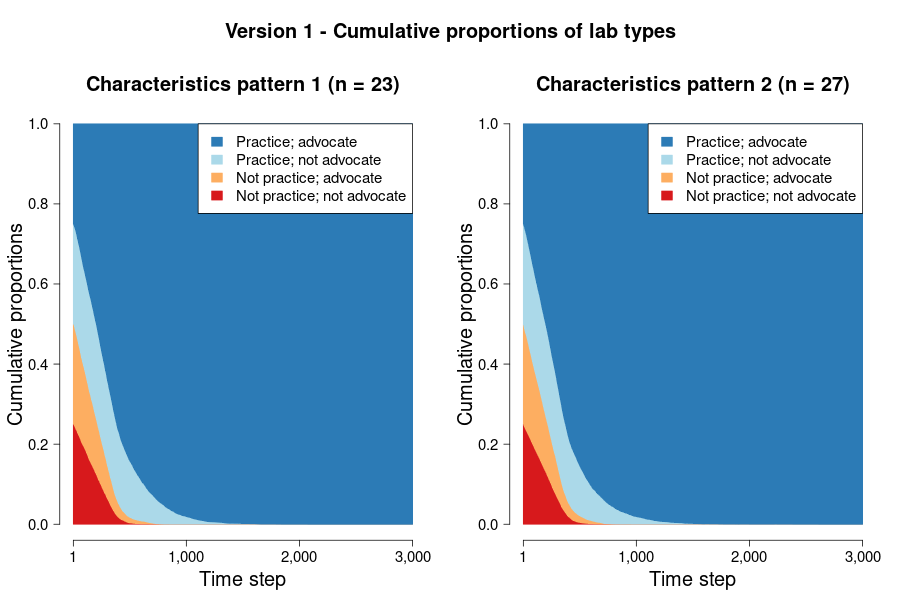
\includegraphics[width=\textwidth]{v1_pro_plot_main.png}
    \caption{Cumulative proportions of lab types during the first $3,000$ out of $1,000,000$ time steps of the first set of simulations. The two panels represent simulation runs with two qualitatively different patterns of characteristics.}
    \label{fig:v1_pro_plot_main}
  \end{fullwidth}
\end{figure*}

As a primary result, we collected data on which lab type(s) survive over time and which die out in a world where everyone ``plays the game''. Specifically, we investigated in what proportions the lab types are present over time: Which lab type(s) is/are most successful within the academic community? As a secondary result, we collected similar data as \textcite{SmaldinoMcelreath2016} about the mean $e$, mean $r$, mean $\alpha$, $FDR$, and mean $W$ across all lab types. For our simulations, we kept $e$ fixed within lab type (see Table~\ref{tab:parameters}).

To reduce the computation time of the simulations, we used a maximum literature size of $100,000$ instead of $1,000,000$. Moreover, we simulated over $1,000,000$ time steps. We sampled every time step for iterations between $1$ and $1,000$ iterations, every $10$th time step for iterations between $1,000$ and $10,000$, every $100$th time step for iterations between $10,000$ and $100,000$, and every $1,000$th time step for iterations between $100,000$ and $1,000,000$.

\subsection{Further Exploration}

We ran an additional set of simulations that incorporated a few more changes to the computational model. First, we reasoned that the payoff for negative novel studies (i.e., $V_{N-}$) should probably not be as high as the payoff for positive novel studies (i.e., $V_{N+}$). In an attempt to get a more informed estimate, we quantified publication advantage using articles published in the New England Journal of Medicine in $2015$. Data was previously extracted by \textcite{HoekstraMondenVanravenzwaaij_2018}. In determining whether a study was considered positive or negative, we focused on statistical inference for the primary outcome. We excluded case studies, descriptive studies, non-inferiority trials, and single-arm studies. Next, we counted all citations (as counted through Google Scholar on date December 9, 2022) for the $120$ positive results papers and the $42$ null result papers. In the past seven years, null result papers were cited a median of $601.5$ times and positive trials were cited a median of $826$ times. The ratio of these two medians is $0.728$ (i.e., positive novel results have a citation advantage of $1$-to-$0.728$). Therefore, we set $V_{N+}=1$ and $V_{N-}=0.728$ for labs that do not practice and do not advocate OS.

Second, the results of the previous simulations suggest that the characteristics of the scientific community have not yet reached a steady state after $1,000,000$ time steps (see Figure~\ref{fig:v1_cha_plot_main}). To investigate this further, we decided to increase the mutation probabilities for $r$ and $W$ from $\mu_r=\mu_W=0.01$ to $\mu_r=\mu_W=0.1$, so that lab characteristics change more quickly.

\section{Results}

Looking at the development of the lab characteristics in the $50$ simulation runs separately, we noticed that individual simulations resulted in one of two qualitatively different patterns of characteristics (i.e., $FDR$, $W$, $\alpha$, and $r$), which are described below. To acknowledge this dichotomy, instead of averaging all $50$ simulation runs, we split them according to the pattern of characteristics observed and averaged them separately. This applies to both the proportions of lab types as well as the community characteristics. Accordingly, for our results, we always provide one plot for simulations that exhibited characteristics pattern $1$ and one plot for simulations that exhibited characteristics pattern $2$.

\begin{figure*}[!t]
  \begin{fullwidth}
    \centering
    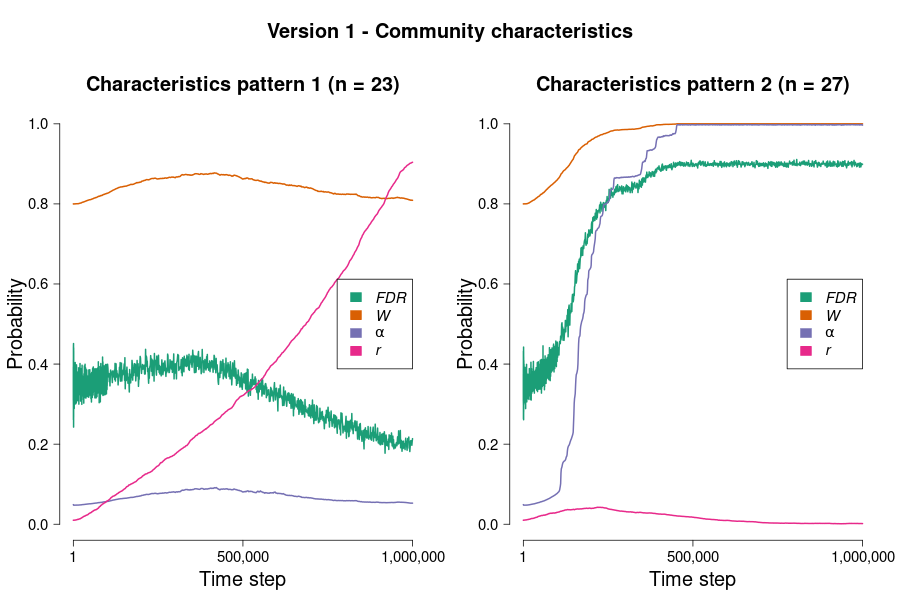
\includegraphics[width=\textwidth]{v1_cha_plot_main.png}
    \caption{Power $W$, false discovery rate $FDR$, false positive rate $\alpha$, and replication probability $r$ averaged over labs and simulation runs over all $1,000,000$ time steps of the first set of simulations. The two panels differentiate between simulation runs with two qualitatively different patterns of characteristics.}
    \label{fig:v1_cha_plot_main}
  \end{fullwidth}
\end{figure*}

\subsection{Who Dominates Science?}

Figure~\ref{fig:v1_pro_plot_main} shows the proportions of the four lab types over the first $3,000$ time steps. The two panels differentiate between simulation runs that displayed two qualitatively different patterns of characteristics, explained in the next section (see also Figure~\ref{fig:v1_cha_plot_main}). Labs that practice and advocate OS reach a proportion of $1$ very quickly; at the same time, the other three lab types vanish. Of those, labs that do not practice OS and do not advocate OS disappear most quickly, followed by labs that do not practice OS but advocate OS and labs that practice OS but do not advocate OS.
%

\begin{figure*}[!t]
  \begin{fullwidth}

    \centering
    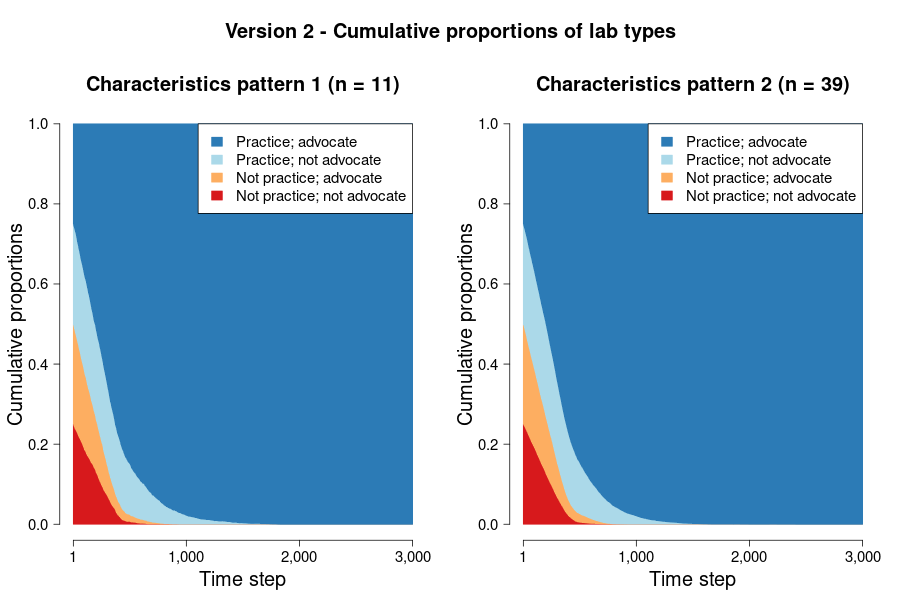
\includegraphics[width=\textwidth]{v2_pro_plot_main.png}
    \caption{Cumulative proportions of lab types during the first $3,000$ out of $1,000,000$ time steps of the first set of simulations. The two panels represent simulation runs with two qualitatively different patterns of characteristics.}
    \label{fig:v2_pro_plot_main}
  \end{fullwidth}
\end{figure*}
%

The observed behavior indicates that practicing OS is more important than advocating OS, but that doing both is most advantageous. This advantage of practicing over advocating holds across the entire range of parameter values we investigated (see Figures~\ref{fig:v1_pro_plot_sens_payypro1.242},~\ref{fig:v1_pro_plot_sens_payypro1.483},~and~\ref{fig:v1_pro_plot_sens_payypro1.725} in Appendix~\ref{sec:appendix_a}). The explanation for this is that there is an additional advantage for labs that practice OS, which is the higher probability of publishing a negative novel finding (i.e., $C_{N-}$, $0.3$ versus $0.05$). Furthermore, the same behavior is observed for various values of $V_{0-}$ ($-5$, $-25$, $-50$, $-100$; see Figure~\ref{fig:v1_pro_plot_vnm} in Appendix~\ref{sec:appendix_b}). In sum, in our evolutionary model the additional cost in terms of increased effort (practicing) and a reduction of work time spent on the actual research (advocating) is easily outweighed by the increased payoff when the work gets published.



\subsection{Characteristics of the Scientific Community}

Figure~\ref{fig:v1_cha_plot_main} shows the development of characteristics across lab types over the whole range of $1,000,000$ time steps. As all lab types except for the ``practice; advocate'' lab type ceased to exist within around $3,000$ time steps, the development of characteristics shown in Figure~\ref{fig:v1_cha_plot_main} almost exclusively reflects the ``practice; advocate'' lab type. Here, simulations can be differentiated by two qualitatively distinct patterns of characteristics. In the left panel, it can be seen that $W$ increases slightly and then decreases very slowly to the initial value. Similarly, $\alpha$ remains fairly constant. $FDR$ rises a bit and then declines over time. Lastly, $r$ increases strongly to almost $1$ in an almost linear fashion. An explanation for this is that $r$ increases to a critical value, at which point the values of $W$ and $\alpha$ do not matter (enough) anymore. Recall that for a replication, the type of result does not matter in terms of payoff. As such, $r$ grows to $1$. In this variant, mutations are such that the certain payoff of replications was higher than the variable payoff of novel results, with a relatively high occurrence of null results. The reader may notice that $W$ does not grow quite so strongly in the first time steps, giving $r$ enough time to gain momentum.
%
%

\begin{figure*}[!t]
  \begin{fullwidth}
    \centering
    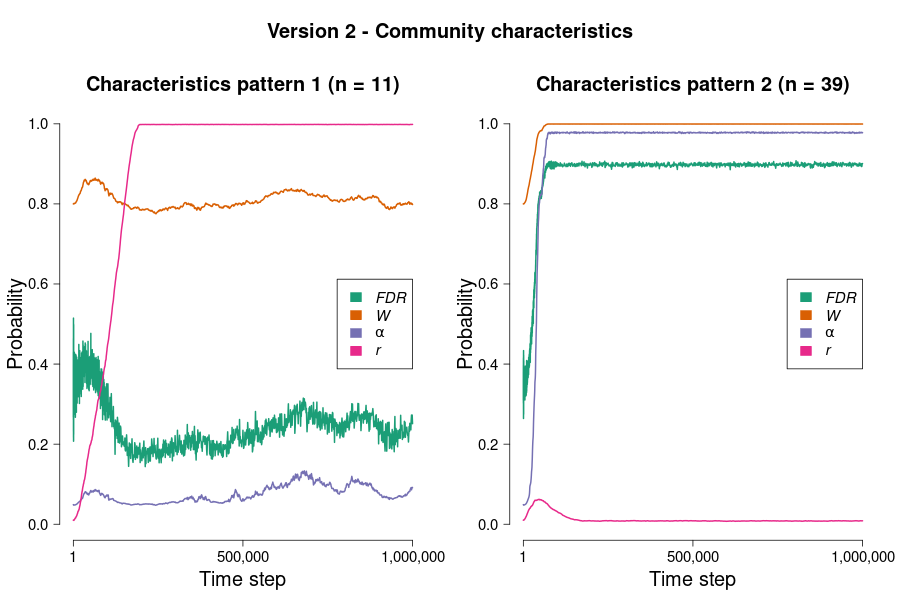
\includegraphics[width=\textwidth]{v2_cha_plot_main.png}
    \caption{Power $W$, false discovery rate $FDR$, false positive rate $\alpha$, and replication probability $r$ averaged over labs and simulation runs over all $1,000,000$ time steps of the second set of simulations. The two panels differentiate between simulation runs with two qualitatively different patterns of characteristics.}
    \label{fig:v2_cha_plot_main}
  \end{fullwidth}
\end{figure*}


The right panel displays entirely different characteristics. Here, both $W$ and $\alpha$ increase rapidly to $1$ and remain constant. $FDR$ also increases strongly but reaches a plateau at around $0.85$. In contrast, $r$ remains very low at almost $0$. The explanation is straightforward: if $W$ and $\alpha$ are $1$, all results are positive results by default, meaning that every lab should conduct novel studies over replications. This is the case because the payoff is double, and there is no drawback. Note that this second pattern of results was not obtained in \cite{KohrtSmaldinoMcelreath_2022preprint} as they fix power in their simulations.



\subsection{Further Exploration}

We further explored the proportions of lab types and the characteristics of the scientific community with some slight parameter modifications: Changing $\mu_W$ and $\mu_r$ from $0.01$ to $0.1$ and changing $V_{N-}$ from $1$ to $0.728$. Figure~\ref{fig:v2_pro_plot_main} shows the proportions of lab types over time. The behavior is very similar to the previous simulations in Figure~\ref{fig:v1_pro_plot_main}, such that labs that practice and advocate OS dominate very quickly while the other lab types die out. Once again, these results are robust to different choices of parameter values (see Figures~\ref{fig:v2_pro_plot_sens_payypro1.242},~\ref{fig:v2_pro_plot_sens_payypro1.483},~and~\ref{fig:v2_pro_plot_sens_payypro1.725} in Appendix~\ref{sec:appendix_a}).

Figure~\ref{fig:v2_cha_plot_main} shows the characteristics of the scientific community. As in the first set of simulations (see Figure~\ref{fig:v1_cha_plot_main}), the characteristics reflect those of the labs that practice and advocate OS through most of the time. As in the first set of simulations, we observed two qualitatively different patterns of characteristics of the labs. The explanation for this is the same as for the first set of simulations (see previous section).
%
%
%
%

\section{Discussion}

Science is not just about the academic work-- it is ultimately a joint enterprise by people. People who depend on their academic position for their livelihood. As such, doing well, or at least doing better than others, on whatever metric is used to evaluate one's success becomes important to people. \textcite{SmaldinoMcelreath2016} demonstrate that if all people do is ``play the game'', the scientific work their field produces over time gradually degenerates to low-effort, quick-and-dirty work with a high proportion of false positives.

The OS movement should restrict the feasibility of some of the quick-and-dirty strategies to which researchers might, inadvertently, fall prey to. For instance, preregistering one's work makes it very difficult to employ $p$-hacking or to hypothesize after the results are known. That said, practicing OS brings with it its own set of success indicators, such as prestige in the field, exclusive funding opportunities, and increased visibility of the work; it may therefore well be optimal to continue to ``play the game'', just with a slightly adjusted set of rules. In other words, exploiting the incentive structure for OS practices might lead to receiving the same advantages as actually practicing OS. In this study, we explored how different types of academics would thrive in a scientific system that values OS practices. Namely, we compared labs that practice or do not practice OS and labs that advocate or do not advocate OS.

In an incentive structure that values OS practices, practicing OS while also advocating OS is most advantageous. Our simulation results suggest that labs that follow OS practices and engage as ``OS advocates'' on Twitter or related social media platforms have a survival advantage. The cost associated with both practicing and preaching in terms of a slower ``rate of completion'' of research projects gets outweighed by the increase in payoff for publications. Within the simulation, only labs that both practiced and advocated OS persisted, all other types quickly vanished from the scientific landscape (i.e., they were less successful in terms of attracting attention and gathering citations).

In our model, advocating OS did not have the same advantages as practicing OS. This was true even in the condition where advocating was worth more than practicing in terms of publication payoff ($73\%$ versus $48\%$, respectively). The likely reason for this lies in the probability of being able to publish negative or null results: in our parameterization, this probability was six times higher for OS work. Many journals that align with OS principles vouch to judge the publishability of a work based on the soundness of the research question, the methodology, and the study protocol. More traditional journals, in addition to these criteria, tend to lean heavily on the (statistical) significance of the results.

Practicing and incentivizing OS practices did not eliminate quick-and-dirty science in our simulation. While we observed slightly lower values for the false discovery rate and false positive rate compared to \textcite{SmaldinoMcelreath2016} and the replication \parencite{KohrtSmaldinoMcelreath_2022preprint}, the values were still considerably high ($0.7$ compared to $>0.8$; but see Appendix~\ref{sec:appendix_a}). Without changing the incentive structure that is currently valuing quantity over quality, OS cannot prevent the rise of quick-and-dirty science. As Simine Vazire once put it \parencite{vazire_open_2020}, OS does not act as quality control itself but enables quality control.

\subsection{Limitations}

Although in our model, practicing and advocating OS practices translated to career advantages, some factors cast doubt on the extent to which these findings translate to the real world. Our operationalization of practicing OS involved (slightly) more work per project and a substantial increase in pay-off per publication. Although our parameter settings were grounded to some extent on previous literature, the exact size will be no more than a rough estimate. Perhaps an increase in workload of, say, $50\%$ would be more realistic than an increase of $5\%$, making the practicing of OS far less attractive for purposes of furthering one's career.

For our operationalization of advocating OS, we assumed that scientists spend two hours of their working weeks on their social media of choice in lieu of working to build and maintain their OS profile. Perhaps two hours is unrealistic and ten hours gets closer to the truth. Or perhaps there is no difference at all in hours spent working between active social media scientists and those that are not active on social media: time on social media could be spent entirely during free time.

Similarly, it can be argued that the payoff advantage for labs that practice and/or advocate OS is too high and that it is unrealistic that the payoff advantage remains constant throughout evolution. It is possible that it is more realistic for the payoff advantage to diminish over time as an increasing amount of conducted studies are OS studies.

An additional limitation is the omission of consideration regarding the potential consequences of disclosing specific research data. Opening up access to such data may facilitate the identification of inaccuracies and provide a basis for heightened scrutiny from the broader research community \parencite{AllenMehler2019}. Theoretically, this increased transparency could adversely affect the sustainability of a research laboratory, particularly if  (unintentional) errors are unveiled and subject to public discourse.

Another, more general, limitation of our setup was the generic classification of scientists as OS practitioners versus non-practitioners and advocators versus non-advocators. In the real world, these categories (and the payoffs they entail) will rarely be so black-and-white. In addition, there will be individual differences in academic success that are tangential to the four categories specified here due to field of interest, background, social network, and even luck. In our simulation, these natural sources of variation were all completely equated. As such, the results of this study should be thought of more as a proof of concept in a drastically simplified representation of what in reality is a very complicated academic ecosphere.

Lastly, our modeling approach to investigate what lab types survive in a community that values open science is only one of many. Different approaches may shed light on the conditions under which labs with different strategies flourish. For instance, using a game theory approach would model the individual labs as rational agents with (potentially) different strategies (e.g., affinity to OS, payoff, etc.). In such an approach, the individual labs would play the ``science game'', which would allow the computation of an equilibrium distribution of different types of labs.

\subsection{Conclusion}

In our simulation, labs that practice and advocate OS thrive in a scientific community that values OS. At the same time, ``quick-and-dirty'' science is still prevalent, as evident by high false positive and false discovery rates. These results are encouraging to those who feel practicing open science ``is not worth it'': in addition to benefits to science at large, our results suggest engaging with OS benefits the individual researcher as well.

\section{Acknowledgements}

We are grateful to Joyce M. Hoek, Jasmine Muradchanian, and Ymkje Anna de Vries for interesting and inspiring discussions.

\section{Protocol, Code, and Data Availability}

A transparency documentation of our research process, the code for the simulations, and the data of the simulations can be found online at \href{https://osf.io/h5tfv/}{https://osf.io/h5tfv/}.

\printbibliography

\newpage
\onecolumn
\appendix

\section{Appendices}
\subsection{A. Sensitivity Analyses for Lab Proportions and Characteristics}\label{sec:appendix_a}

For all sensitivity analyses, we did not differentiate between simulation runs with two qualitatively different patterns of characteristics (see Results section). Instead, we averaged over all simulation runs. Each of the following Figures contains various parameter combinations. One additional parameter (i.e., the payoff advantage for advocating OS $\gamma$) differentiates between Figures. Figures~\ref{fig:v1_pro_plot_sens_payypro1.242},~\ref{fig:v1_pro_plot_sens_payypro1.483},~and~\ref{fig:v1_pro_plot_sens_payypro1.725} show the lab proportions for the first set of simulations with payoff advantages for advocating OS of $\gamma=\left\{1.242, 1.483, 1.725\right\}$, respectively; Figures~\ref{fig:v1_cha_plot_sens_payypro1.242},~\ref{fig:v1_cha_plot_sens_payypro1.483},~and~\ref{fig:v1_cha_plot_sens_payypro1.725} show the community characteristics for the first set of simulations with payoff advantages for advocating OS of $\gamma=\left\{1.242, 1.483, 1.725\right\}$, respectively. Similarly, Figures~\ref{fig:v2_pro_plot_sens_payypro1.242},~\ref{fig:v2_pro_plot_sens_payypro1.483},~and~\ref{fig:v2_pro_plot_sens_payypro1.725} show the lab proportions for the second set of simulations with payoff advantages for advocating OS of $\gamma=\left\{1.242, 1.483, 1.725\right\}$, respectively; Figures~\ref{fig:v2_cha_plot_sens_payypro1.242},~\ref{fig:v2_cha_plot_sens_payypro1.483},~and~\ref{fig:v2_cha_plot_sens_payypro1.725} show the community characteristics for the second set of simulations with payoff advantages for advocating OS of $\gamma=\left\{1.242, 1.483, 1.725\right\}$, respectively.

Figures~\ref{fig:v1_pro_plot_sens_payypro1.242},~\ref{fig:v1_pro_plot_sens_payypro1.483},~\ref{fig:v1_pro_plot_sens_payypro1.725},~\ref{fig:v2_pro_plot_sens_payypro1.242},~\ref{fig:v2_pro_plot_sens_payypro1.483},~and~\ref{fig:v2_pro_plot_sens_payypro1.725} clearly demonstrate that the lab proportions are robust against specific choices of parameter combinations. In all cases, the ``practice; advocate'' lab type wins and suppresses the other lab types. Although there is more variation in the community characteristics for different parameter combinations (see Figures~\ref{fig:v1_cha_plot_sens_payypro1.242},~\ref{fig:v1_cha_plot_sens_payypro1.483},~\ref{fig:v1_cha_plot_sens_payypro1.725},~\ref{fig:v2_cha_plot_sens_payypro1.242},~\ref{fig:v2_cha_plot_sens_payypro1.483},~and~\ref{fig:v2_cha_plot_sens_payypro1.725}), the overall trends are still quite robust.
%
\begin{figure*}
  \begin{fullwidth}

    \centering
    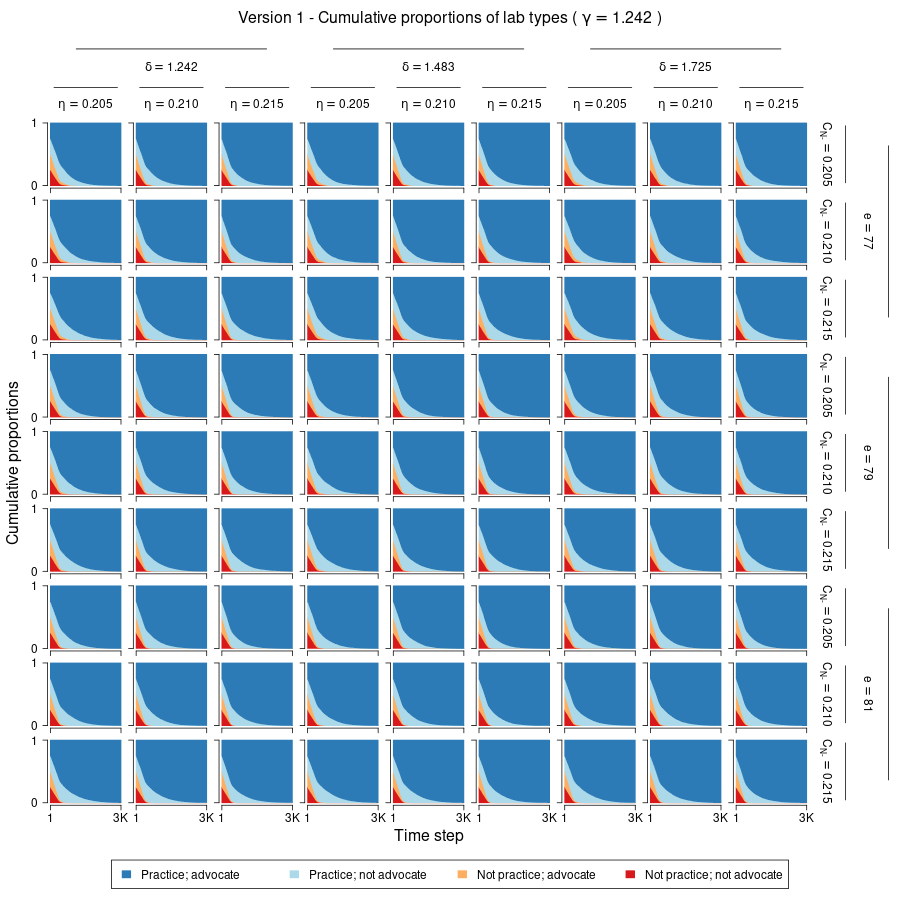
\includegraphics[width=\textwidth]{v1_pro_plot_sens_payypro1.242.png}
    \caption{Cumulative proportions of lab types during the first $3,000$ out of $1,000,000$ time steps of the first set of simulations with $\gamma=1.242$ and different parameter combinations. Note that panels show an average of all $50$ simulation runs. $\gamma$ and $\delta$ are the payoff advantages for advocating and practicing OS, respectively.}
    \label{fig:v1_pro_plot_sens_payypro1.242}
  \end{fullwidth}
\end{figure*}
%
%
\begin{figure*}
  \begin{fullwidth}
    \centering
    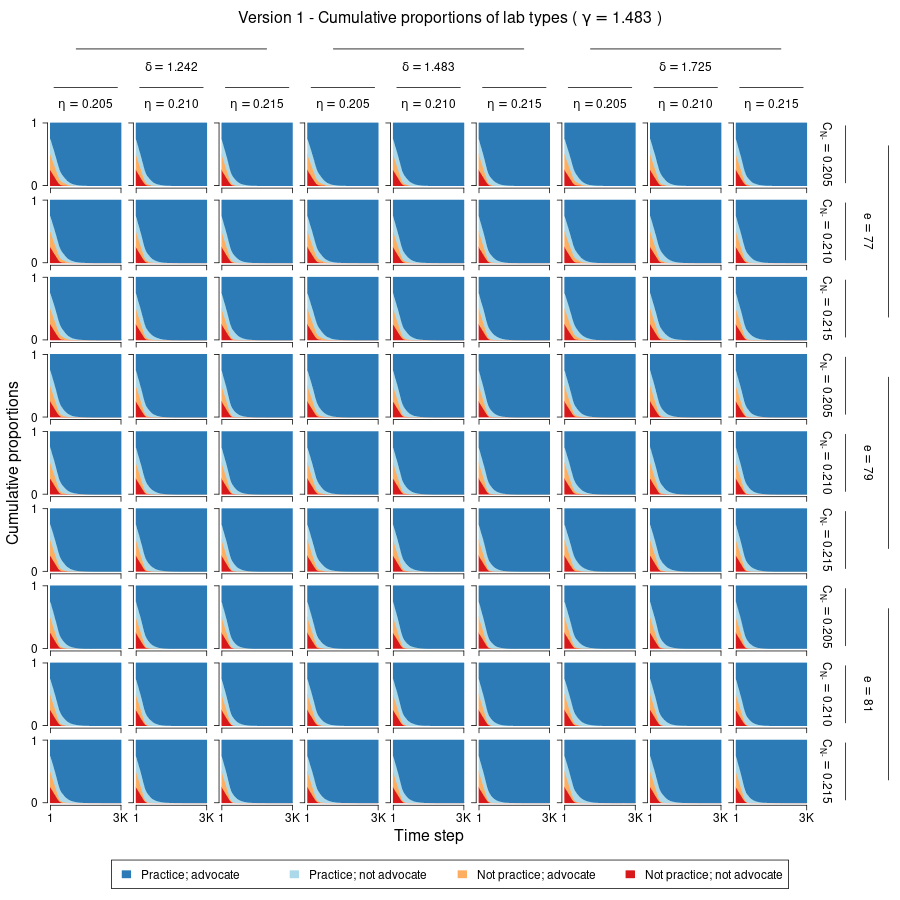
\includegraphics[width=\textwidth]{v1_pro_plot_sens_payypro1.483.png}
    \caption{Cumulative proportions of lab types during the first $3,000$ out of $1,000,000$ time steps of the first set of simulations with $\gamma=1.483$ and different parameter combinations. Note that panels show an average of all $50$ simulation runs. $\gamma$ and $\delta$ are the payoff advantages for advocating and practicing OS, respectively.}
    \label{fig:v1_pro_plot_sens_payypro1.483}
  \end{fullwidth}
\end{figure*}
%
%
\begin{figure*}
  \begin{fullwidth}
    \centering
    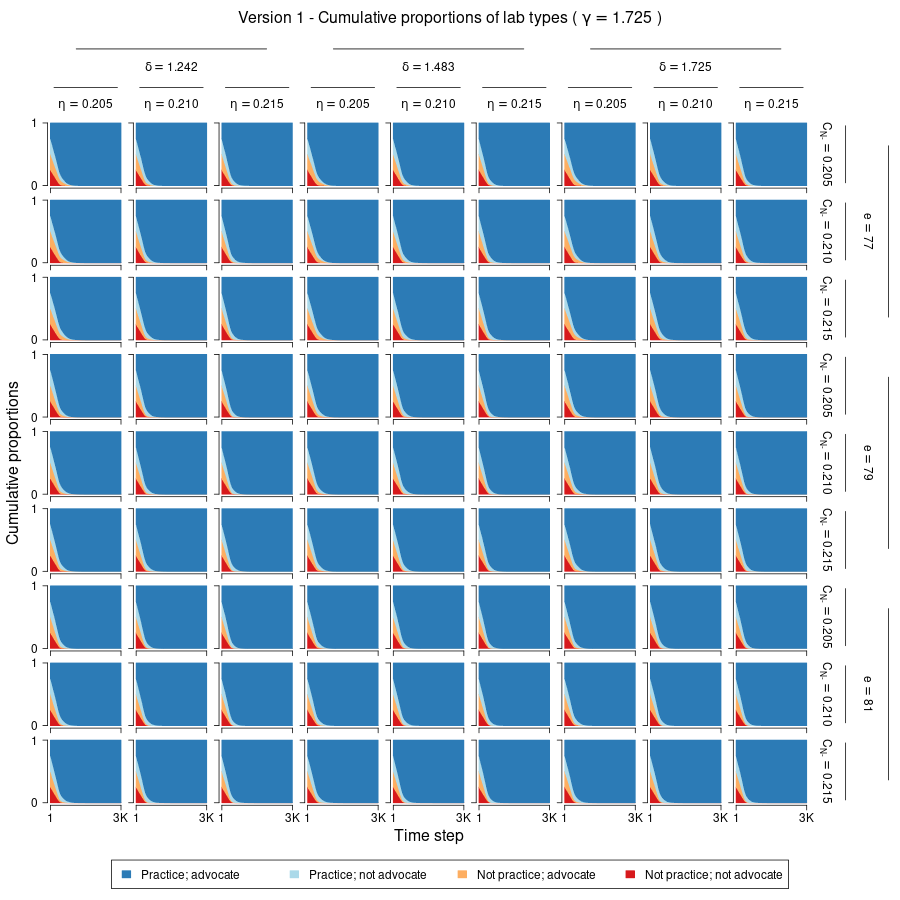
\includegraphics[width=\textwidth]{v1_pro_plot_sens_payypro1.725.png}
    \caption{Cumulative proportions of lab types during the first $3,000$ out of $1,000,000$ time steps of the first set of simulations with $\gamma=1.725$ and different parameter combinations. Note that panels show an average of all $50$ simulation runs. $\gamma$ and $\delta$ are the payoff advantages for advocating and practicing OS, respectively.}
    \label{fig:v1_pro_plot_sens_payypro1.725}
  \end{fullwidth}
\end{figure*}
%
%
\begin{figure*}
  \begin{fullwidth}
    \centering
    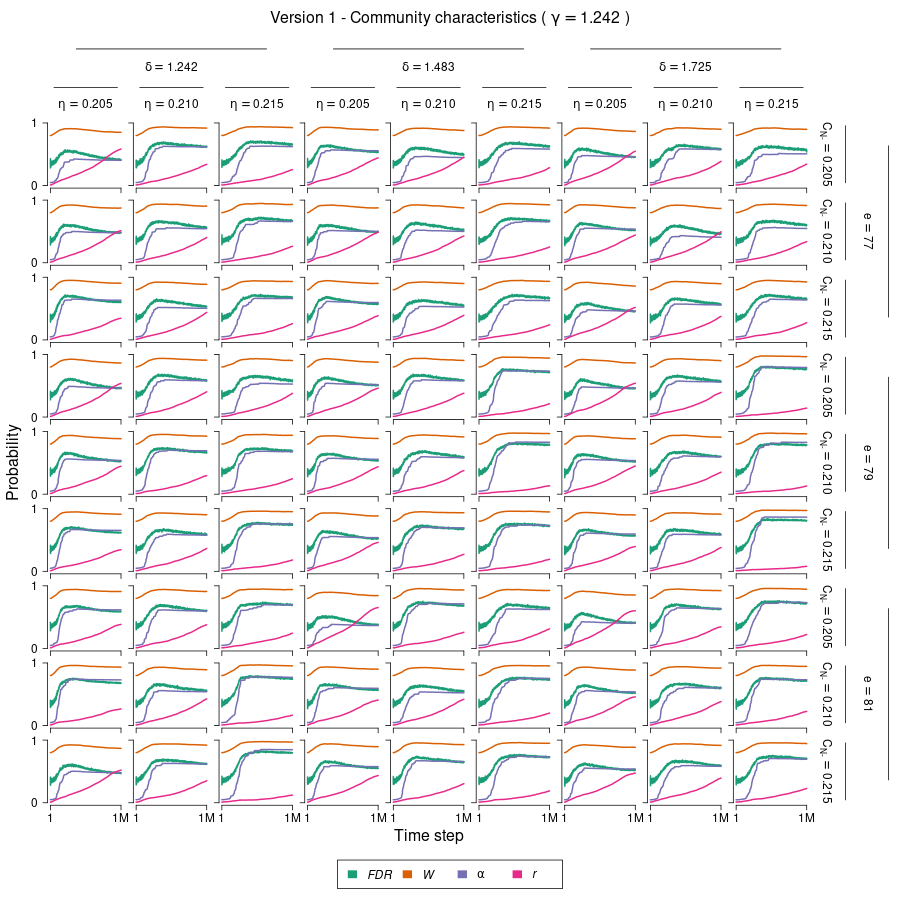
\includegraphics[width=\textwidth]{v1_cha_plot_sens_payypro1.242.png}
    \caption{Power $W$, false discovery rate $FDR$, false positive rate $\alpha$, and replication probability $r$ averaged over all labs over all $1,000,000$ time steps of the first set of simulations with $\gamma=1.242$ and different parameter combinations. Note that panels show an average of all $50$ simulation runs. $\gamma$ and $\delta$ are the payoff advantages for advocating and practicing OS, respectively.}
    \label{fig:v1_cha_plot_sens_payypro1.242}
  \end{fullwidth}
\end{figure*}
%
%
\begin{figure*}
  \begin{fullwidth}
    \centering
    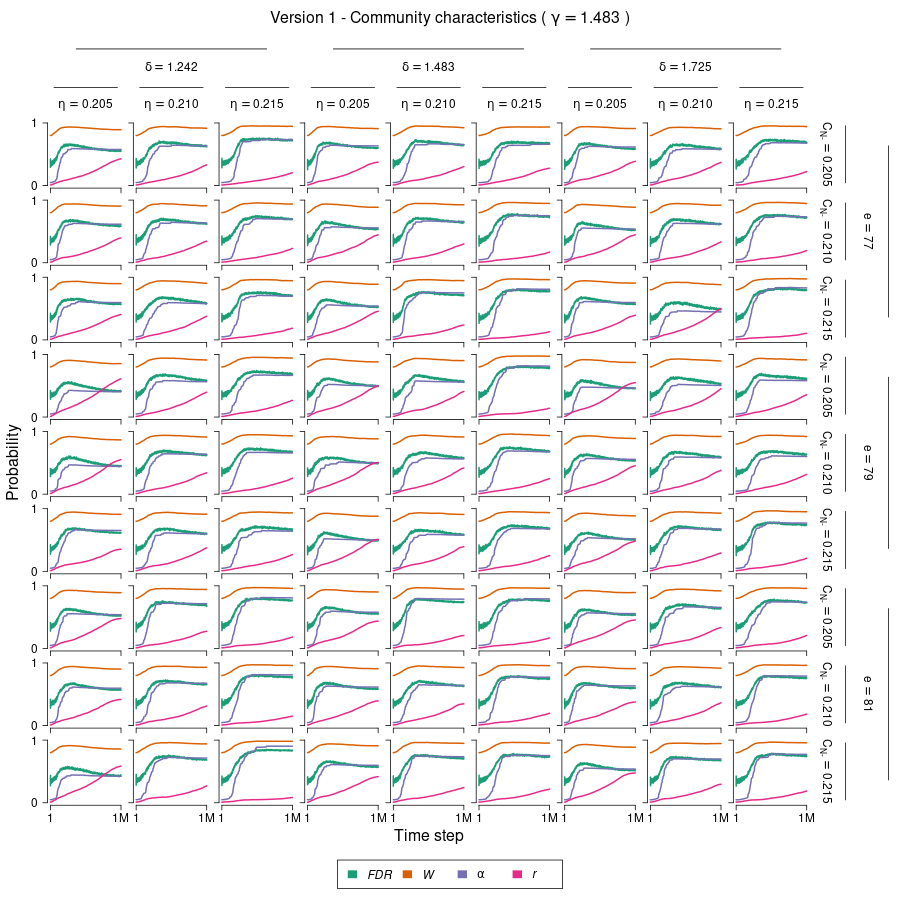
\includegraphics[width=\textwidth]{v1_cha_plot_sens_payypro1.483.png}
    \caption{Power $W$, false discovery rate $FDR$, false positive rate $\alpha$, and replication probability $r$ averaged over all labs over all $1,000,000$ time steps of the first set of simulations with $\gamma=1.483$ and different parameter combinations. Note that panels show an average of all $50$ simulation runs. $\gamma$ and $\delta$ are the payoff advantages for advocating and practicing OS, respectively.}
    \label{fig:v1_cha_plot_sens_payypro1.483}
  \end{fullwidth}
\end{figure*}
%
%
\begin{figure*}
  \begin{fullwidth}
    \centering
    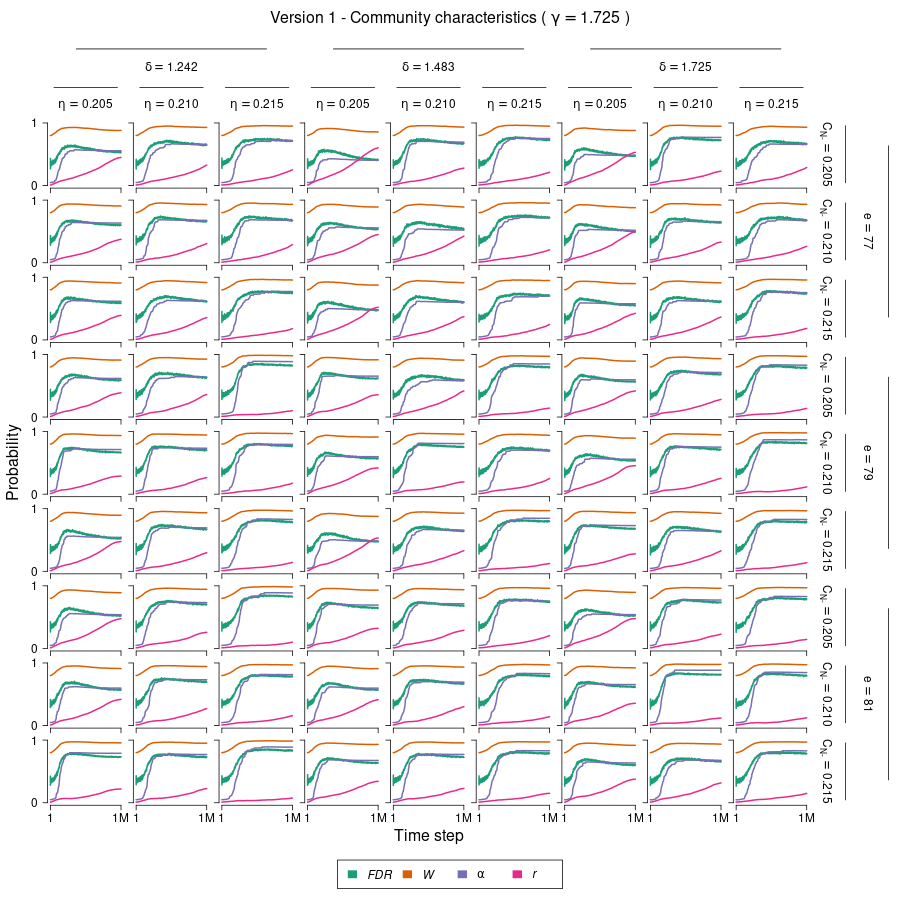
\includegraphics[width=\textwidth]{v1_cha_plot_sens_payypro1.725.png}
    \caption{Power $W$, false discovery rate $FDR$, false positive rate $\alpha$, and replication probability $r$ averaged over all labs over all $1,000,000$ time steps of the first set of simulations with $\gamma=1.725$ and different parameter combinations. Note that panels show an average of all $50$ simulation runs. $\gamma$ and $\delta$ are the payoff advantages for advocating and practicing OS, respectively.}
    \label{fig:v1_cha_plot_sens_payypro1.725}
  \end{fullwidth}
\end{figure*}
%
%
\begin{figure*}
  \begin{fullwidth}
    \centering
    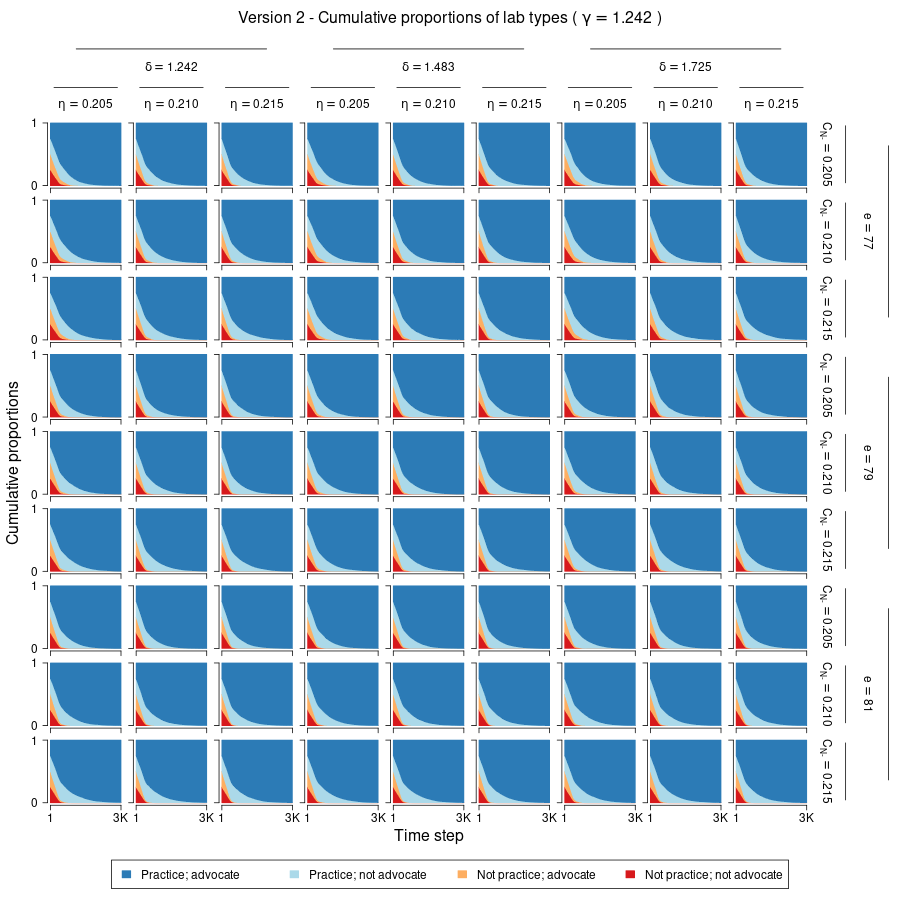
\includegraphics[width=\textwidth]{v2_pro_plot_sens_payypro1.242.png}
    \caption{Cumulative proportions of lab types during the first $3,000$ out of $1,000,000$ time steps of the second set of simulations with $\gamma=1.242$ and different parameter combinations. Note that panels show an average of all $50$ simulation runs. $\gamma$ and $\delta$ are the payoff advantages for advocating and practicing OS, respectively.}
    \label{fig:v2_pro_plot_sens_payypro1.242}
  \end{fullwidth}
\end{figure*}
%
%
\begin{figure*}
  \begin{fullwidth}
    \centering
    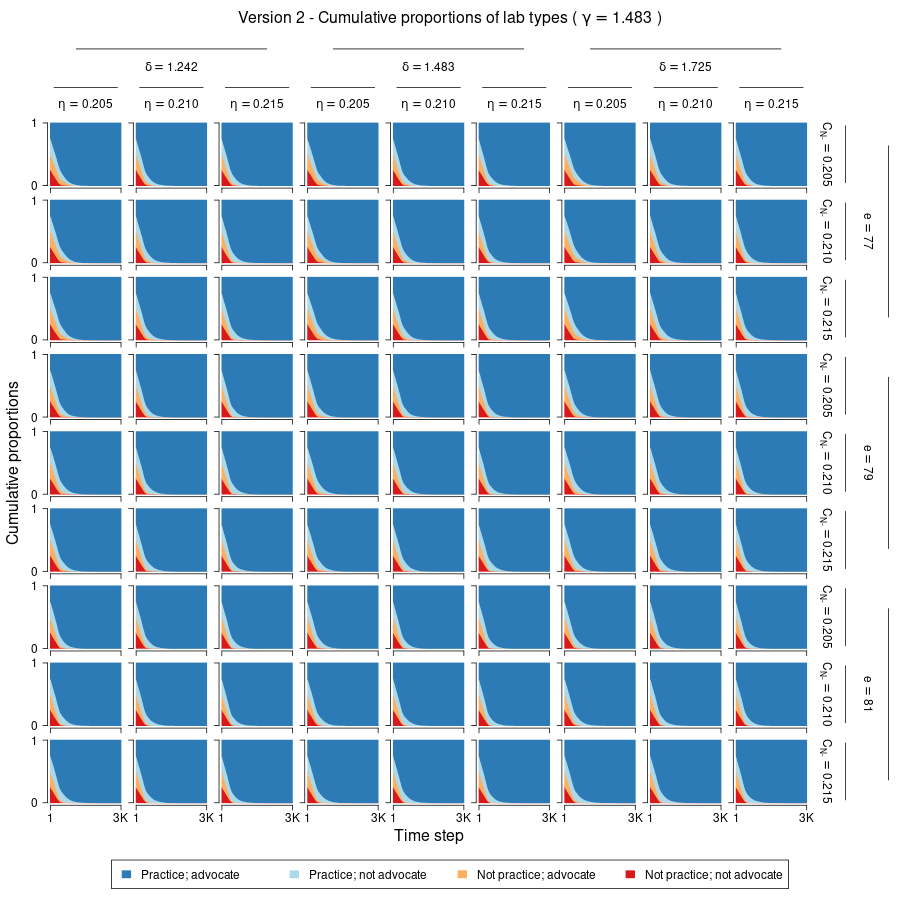
\includegraphics[width=\textwidth]{v2_pro_plot_sens_payypro1.483.png}
    \caption{Cumulative proportions of lab types during the first $3,000$ out of $1,000,000$ time steps of the second set of simulations with $\gamma=1.483$ and different parameter combinations. Note that panels show an average of all $50$ simulation runs. $\gamma$ and $\delta$ are the payoff advantages for advocating and practicing OS, respectively.}
    \label{fig:v2_pro_plot_sens_payypro1.483}
  \end{fullwidth}
\end{figure*}
%
%
\begin{figure*}
  \begin{fullwidth}
    \centering
    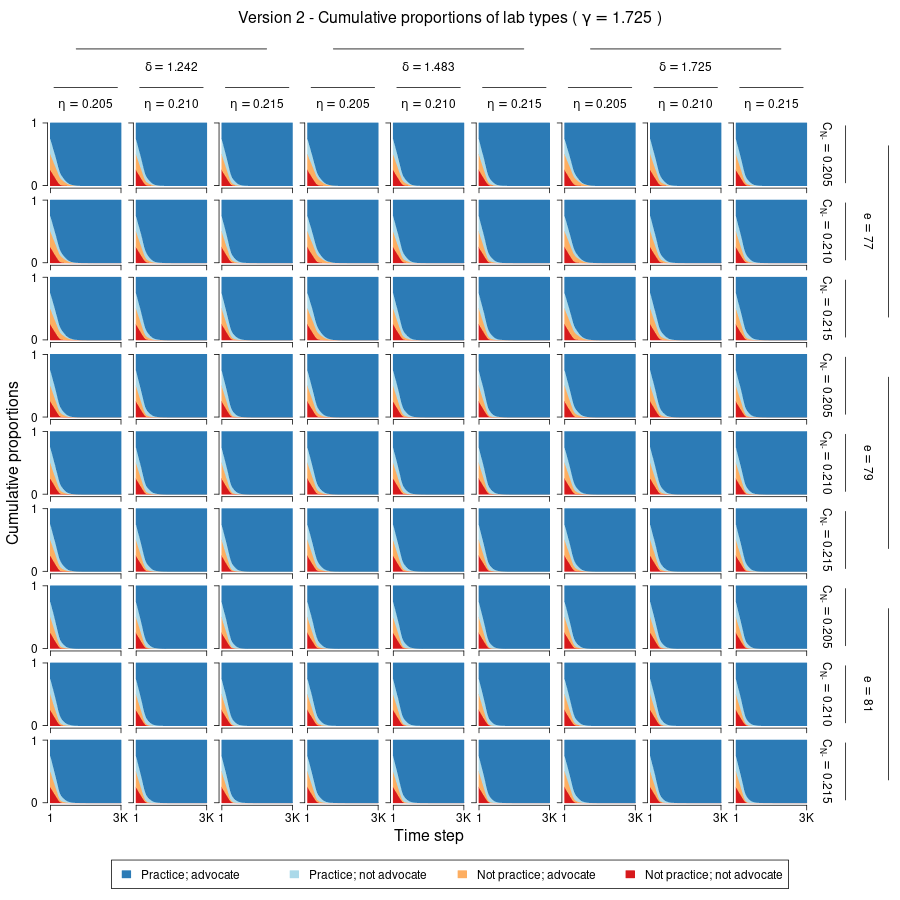
\includegraphics[width=\textwidth]{v2_pro_plot_sens_payypro1.725.png}
    \caption{Cumulative proportions of lab types during the first $3,000$ out of $1,000,000$ time steps of the second set of simulations with $\gamma=1.725$ and different parameter combinations. Note that panels show an average of all $50$ simulation runs. $\gamma$ and $\delta$ are the payoff advantages for advocating and practicing OS, respectively.}
    \label{fig:v2_pro_plot_sens_payypro1.725}
  \end{fullwidth}
\end{figure*}
%
%
\begin{figure*}
  \begin{fullwidth}
    \centering
    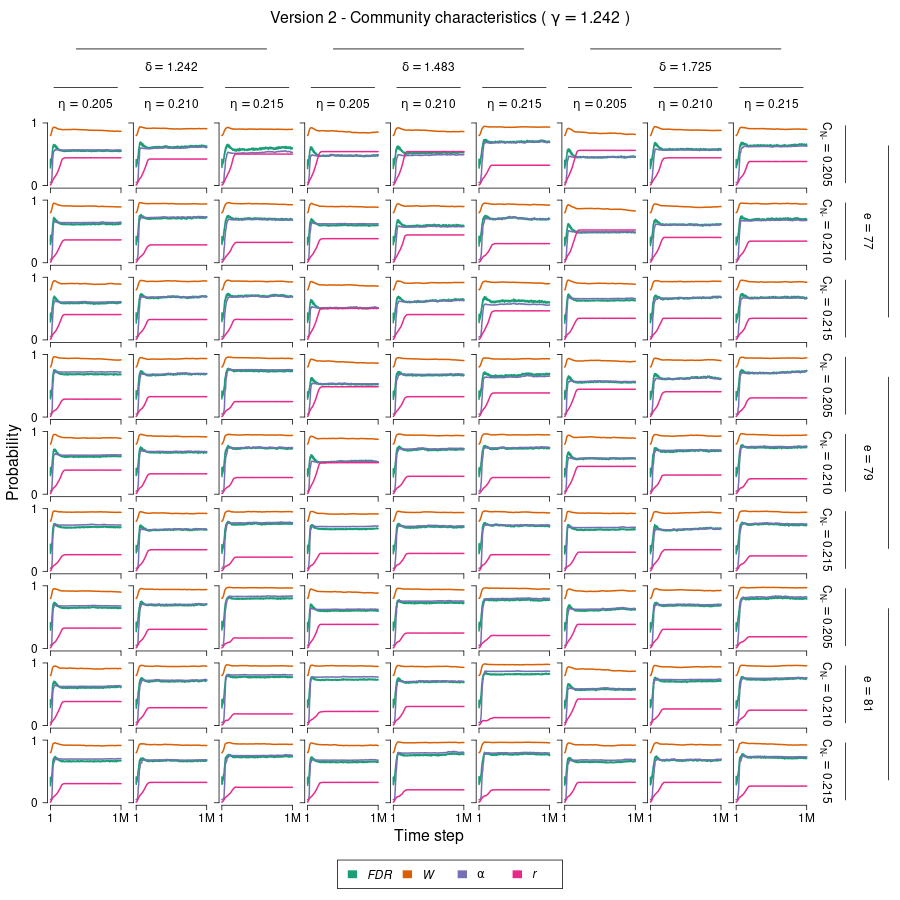
\includegraphics[width=\textwidth]{v2_cha_plot_sens_payypro1.242.png}
    \caption{Power $W$, false discovery rate $FDR$, false positive rate $\alpha$, and replication probability $r$ averaged over all labs over all $1,000,000$ time steps of the second set of simulations with $\gamma=1.242$ and different parameter combinations. Note that panels show an average of all $50$ simulation runs. $\gamma$ and $\delta$ are the payoff advantages for advocating and practicing OS, respectively.}
    \label{fig:v2_cha_plot_sens_payypro1.242}
  \end{fullwidth}
\end{figure*}
%
%
\begin{figure*}
  \begin{fullwidth}
    \centering
    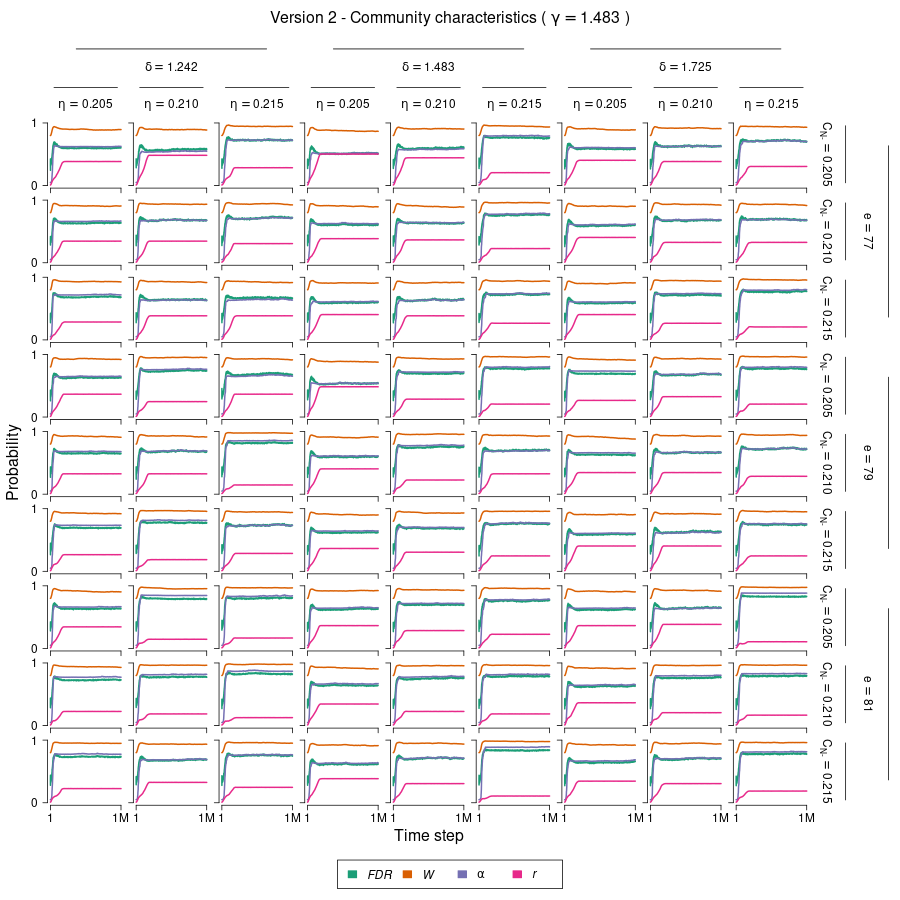
\includegraphics[width=\textwidth]{v2_cha_plot_sens_payypro1.483.png}
    \caption{Power $W$, false discovery rate $FDR$, false positive rate $\alpha$, and replication probability $r$ averaged over all labs over all $1,000,000$ time steps of the second set of simulations with $\gamma=1.483$ and different parameter combinations. Note that panels show an average of all $50$ simulation runs. $\gamma$ and $\delta$ are the payoff advantages for advocating and practicing OS, respectively.}
    \label{fig:v2_cha_plot_sens_payypro1.483}
  \end{fullwidth}
\end{figure*}
%
%
\begin{figure*}
  \begin{fullwidth}
    \centering
    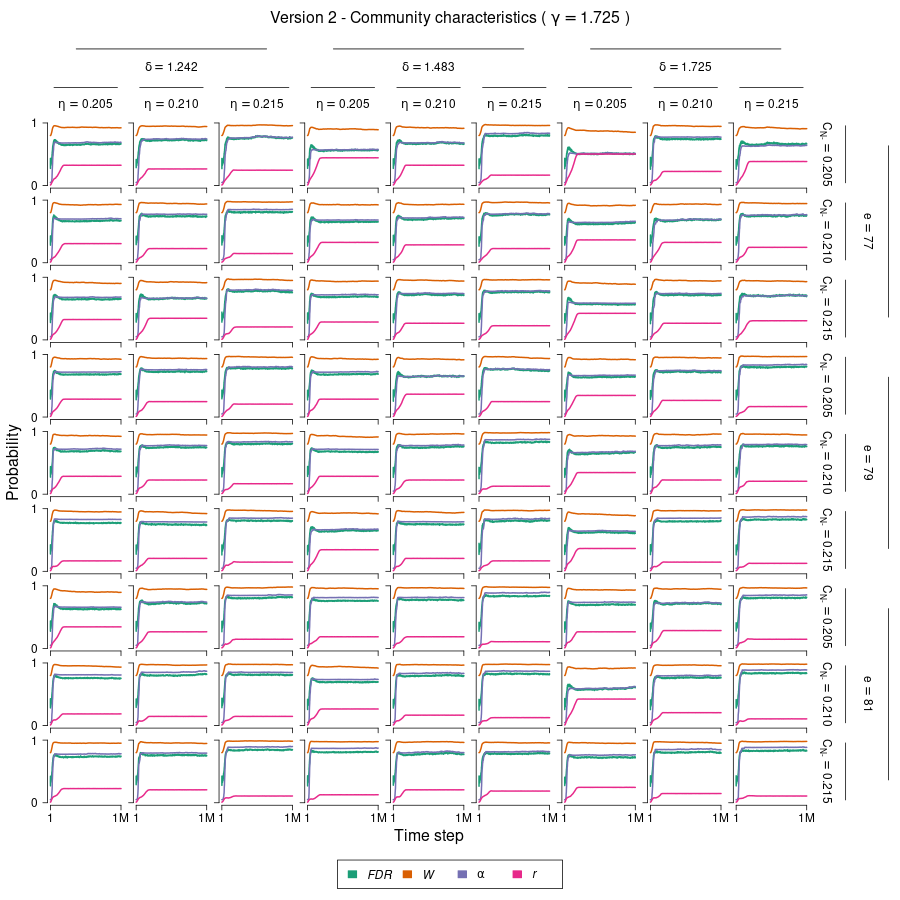
\includegraphics[width=\textwidth]{v2_cha_plot_sens_payypro1.725.png}
    \caption{Power $W$, false discovery rate $FDR$, false positive rate $\alpha$, and replication probability $r$ averaged over all labs over all $1,000,000$ time steps of the second set of simulations with $\gamma=1.725$ and different parameter combinations. Note that panels show an average of all $50$ simulation runs. $\gamma$ and $\delta$ are the payoff advantages for advocating and practicing OS, respectively.}
    \label{fig:v2_cha_plot_sens_payypro1.725}
  \end{fullwidth}
\end{figure*}
%

\clearpage
\subsection{B. Lab proportions and characteristics as a function of $V_{0-}$}\label{sec:appendix_b}

For these additional sensitivity analyses, we did not differentiate between simulation runs with two qualitatively different patterns of characteristics (see Results section). Instead, we averaged over all simulation runs. Figure~\ref{fig:v1_pro_plot_vnm} shows the lab proportions for the first set of simulations as a function of $V_{0-}$ and Figure~\ref{fig:v1_cha_plot_vnm} shows the community characteristics for the first set of simulations as a function of $V_{0-}$. All parameter values, except for $V_{0-}$ are fixed at the values that were used in the main analyses (see Table~\ref{tab:parameters}). Figure~\ref{fig:v1_pro_plot_vnm} clearly demonstrates that the lab proportions are robust against specific choice of $V_{0-}$. Figure~\ref{fig:v1_cha_plot_vnm} shows that the development of $FDR$, $W$, and $\alpha$ is also robust against variations of $V_{0-}$; all of them increase quickly and remain at a high level. However, it can be seen that $r$ increases more strongly the higher the value for $V_{0-}$.
%
\begin{figure*}
  \begin{fullwidth}
    \centering
    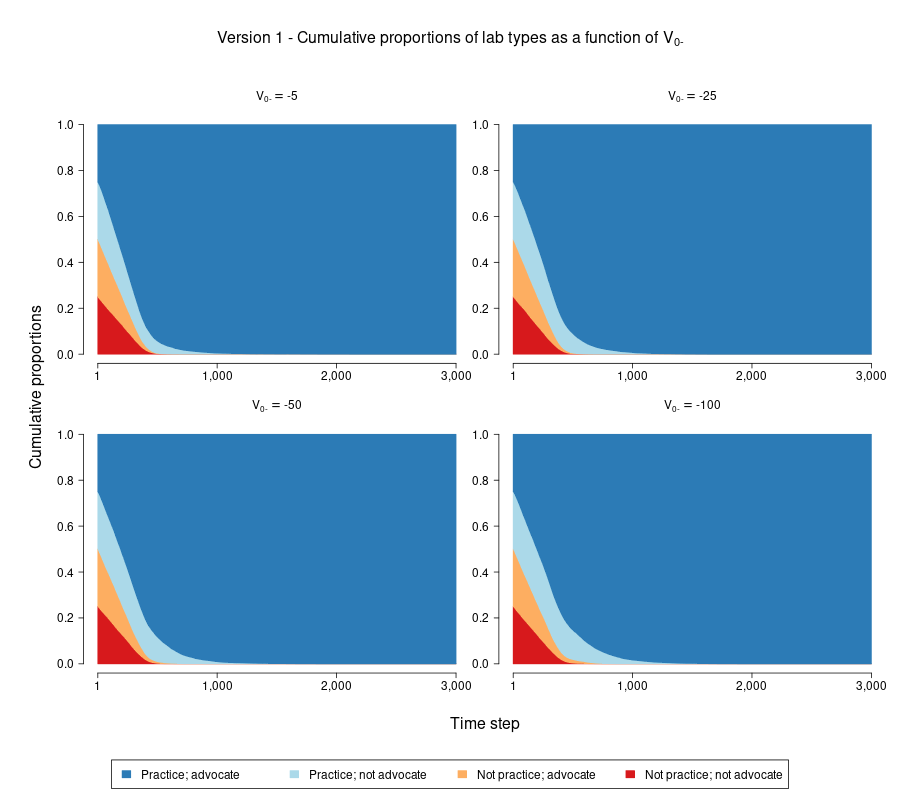
\includegraphics[width=\textwidth]{v1_pro_plot_vnm.png}
    \caption{Cumulative proportions of lab types as a function of $V_{0-}$ during the first $3,000$ out of $1,000,000$ time steps of the first set of simulations. The panels correspond to different values of $V_{0-}$. All other parameter values are fixed at the values that were used in the main analyses (see Table~\ref{tab:parameters}). Note that panels show an average of all $50$ simulation runs.}
    \label{fig:v1_pro_plot_vnm}
  \end{fullwidth}
\end{figure*}
%
%
\begin{figure*}
  \begin{fullwidth}
    \centering
    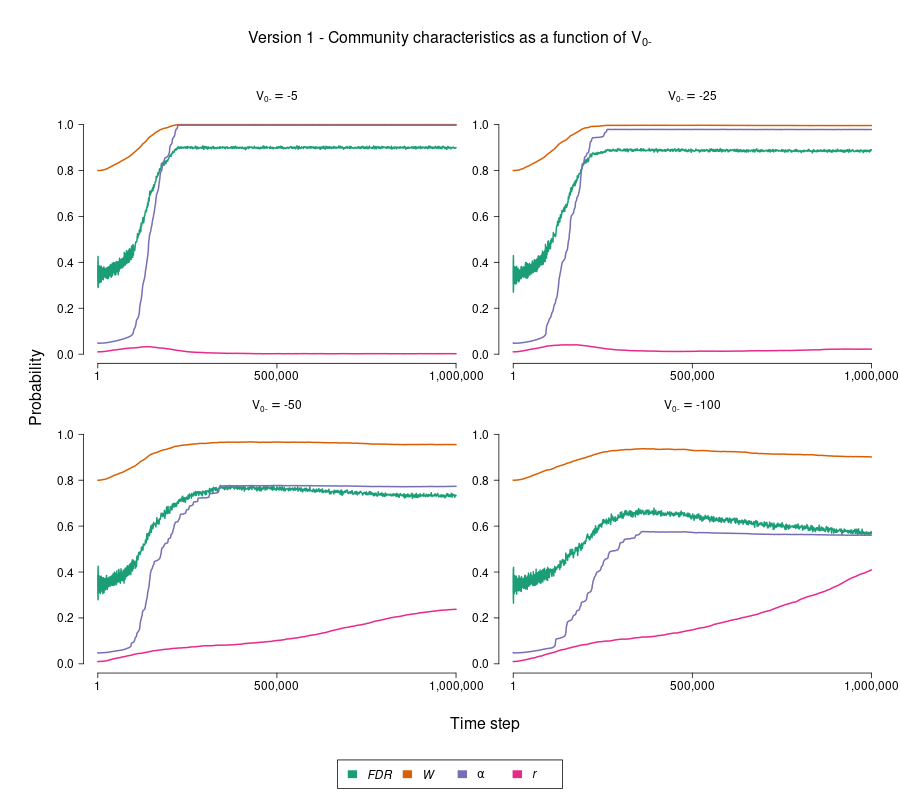
\includegraphics[width=\textwidth]{v1_cha_plot_vnm.png}
    \caption{Power $W$, false discovery rate $FDR$, false positive rate $\alpha$, and replication probability $r$ averaged over all labs as a function of $V_{0-}$ over all $1,000,000$ time steps of the first set of simulations. The panels correspond to different values of $V_{0-}$. All other parameter values are fixed at the values that were used in the main analyses (see Table~\ref{tab:parameters}). Note that panels show an average of all $50$ simulation runs.}
    \label{fig:v1_cha_plot_vnm}
  \end{fullwidth}
\end{figure*}
%

\end{document}
